\chapter{実験2 -光沢感と明るさ感の関連性-}

    \section{目的}

        実験2では,実験1で使用した刺激と同じ色度を持つ単色パッチを用いて,H-K効果,すなわち色度による明るさ感の変化を用いて明るさを定量化する.
        実験1の色度による光沢感の変化と,実験2で計測される色度による明るさ感の変化を比較することで,色度による明るさ感の変化が光沢感に影響を及ぼした可能性について検討する.


    \section{実験方法}
        \subsection{実験環境,被験者}

            実験2で用いた装置と参加した被験者は,いずれも実験1と同一であった.

        \subsection{実験刺激}

            \begin{figure}[h]
                \centering
                
\includegraphics[width=14.0cm]{./img/ex2_stimuli2.png}
                \caption{実験刺激の例}
                \label{ex2_stimuli}
            \end{figure}

            \begin{figure}[h]
                \centering
                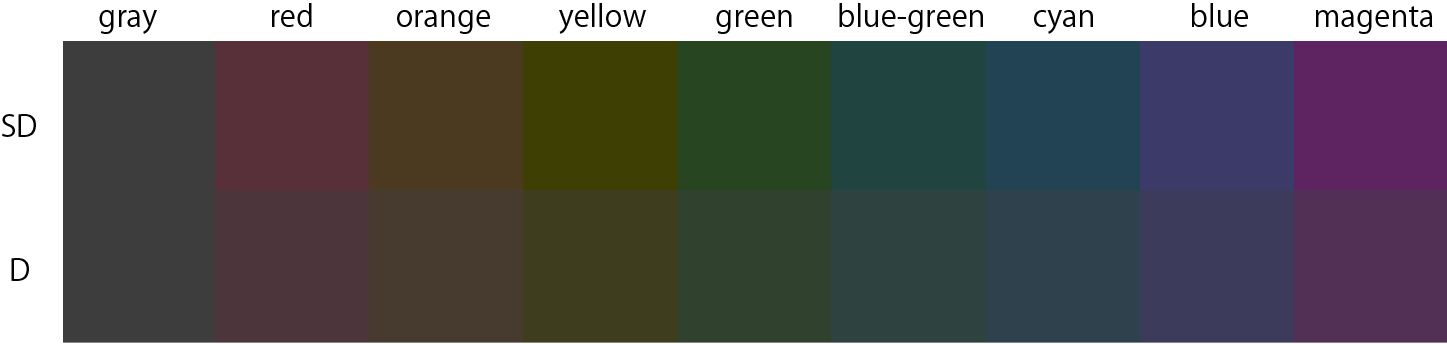
\includegraphics[width=14.0cm]{./img/ex2_stimuli_p.png}
                \caption{参照刺激として使われた色}
                \label{ex2_stimuli_set}
            \end{figure}
            \newpage

            実験2で使用する刺激と,参照刺激に使われた色を図\ref{ex2_stimuli}と図\ref{ex2_stimuli_set}に示す.
            参照刺激として使われた18種類の色度は,実験1で用いたDragon形状におけるSD条件,D条件のそれぞれの刺激の$XYZ$平均色に対応する.
            その輝度は,いずれの色度,彩色条件において5.80 ${\rm cd/m}^2$であった.

        \subsection{実験手続き}

            \begin{figure}[h]
                \centering
                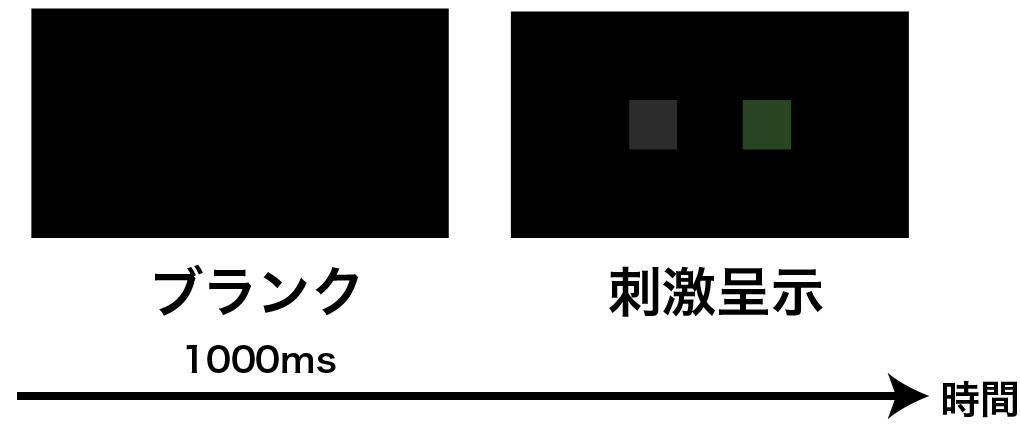
\includegraphics[width=10.0cm]{./img/ex2_procedure.png}
                \caption{1試行の流れ}
                \label{ex2_procedure}
            \end{figure}

            実験2では調整法によりカラーパッチの知覚的な明るさを計測する.
            実験2の1試行の流れを図\ref{ex2_procedure}に示す.
            各試行では,はじめに黒背景のみからなるブランク画面が1000 msの間呈示された.
            次に,参照刺激であるカラーパッチとテスト刺激である無彩色パッチからなる刺激対が呈示された.
            この間に被験者はトラックボールを左右に回すことにより,無彩色パッチの輝度を調節でき,カラーパッチと同じ明るさに知覚されるようになるまで操作した.
            調整に満足したら,トラックボールマウスの右クリックを押すことでその結果が記録され,そのまま次の試行のブランク画面へ移行した.
            なお,カラーパッチと無彩色パッチの左右位置は試行ごとにランダムに決定された.

            各セッションは2彩色条件$\times$色度9通り=18試行からなり,各被験者は全体で5セッションの実験を行った.
            これにより,各被験者は刺激ごとに5試行ずつ行ったことになる.
            また,各セッションの18試行で使われる参照刺激はランダムな順序で選ばれた.

    \section{実験結果}

        \subsection{H-K効果の大きさ}

            \begin{figure}[h]
                \centering
                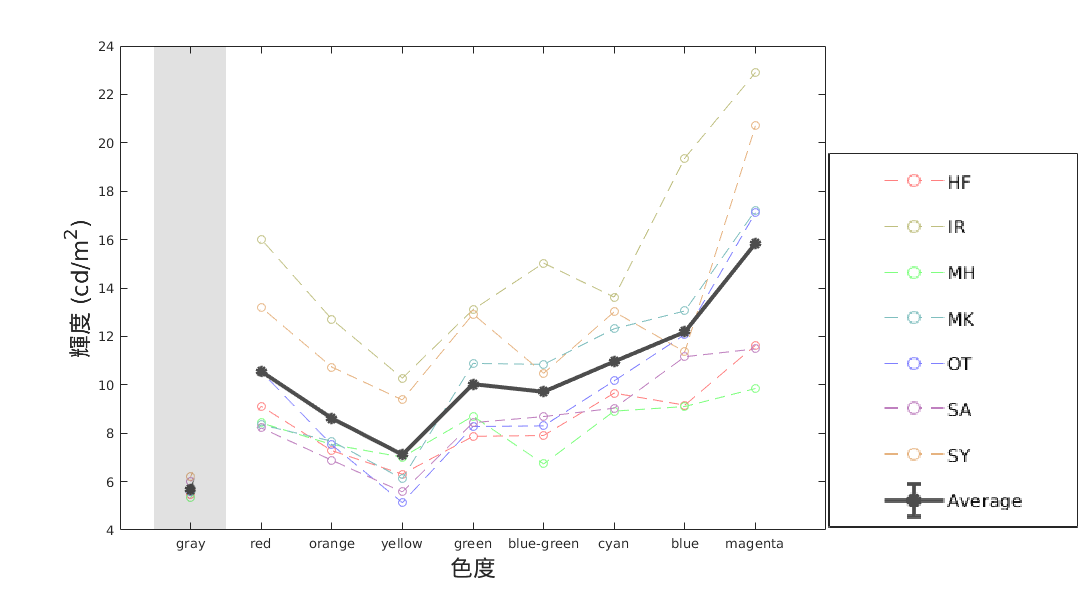
\includegraphics[width=14.0cm]{./img/ex2_res_SD_p.png}
                \caption{SD条件におけるテスト刺激の輝度}
                \label{ex2_SD}
            \end{figure}

            \begin{figure}[h]
                \centering
                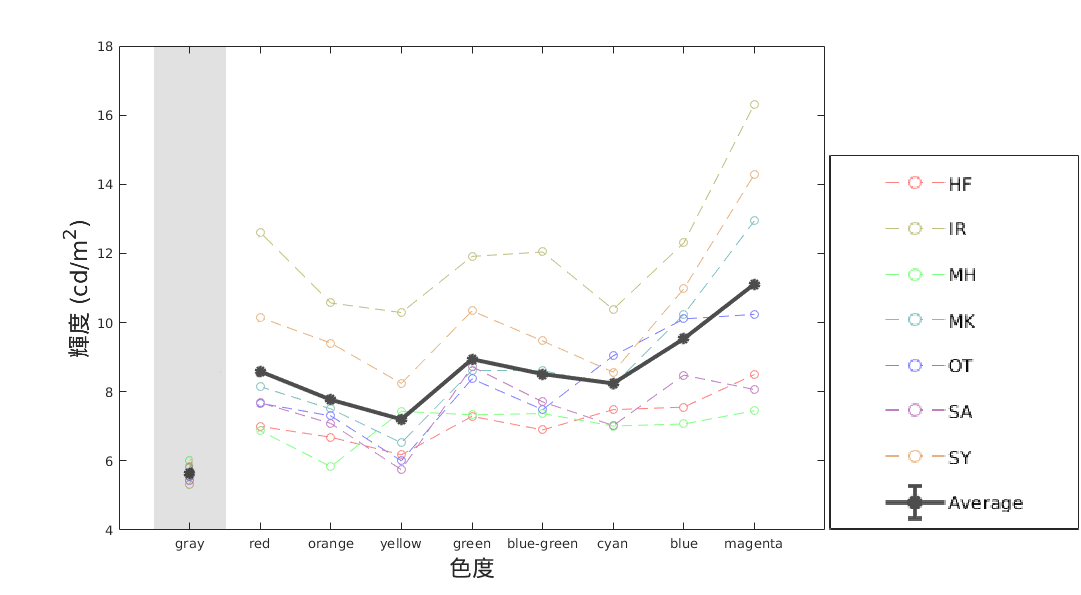
\includegraphics[width=14.0cm]{./img/ex2_res_D_p.png}
                \caption{D条件におけるテスト刺激の輝度}
                \label{ex2_D}
            \end{figure}

            図\ref{ex2_SD}がSD条件の結果,図\ref{ex2_D}がD条件の結果を示す.
            それぞれのグラフにおいて,横軸が刺激色,縦軸が被験者が調整したテスト刺激の輝度を示す.
            また,破線は被験者ごとの結果を表し,色が各被験者に対応している.
            黒実線は被験者間平均の結果を表す.
            これらのグラフにおいて,左端のgrayに対する応答結果がH-K効果がほぼ全く働かない条件であるため,grayとその他の色度の輝度値の差がH-K効果の大きさということになる.
            
            まず,SD条件とD条件のどちらにおいても,すべての色度においてgrayよりも輝度値が大きく,H-K効果が生じたことがわかる.
            その中でも,特にmagentaの輝度が非常に高く,強いH-K効果が生じた.
            一方でyellowでは,grayに次いで輝度が小さく,H-K効果が弱いことがわかる.
            各個人の結果に着目しても,SD条件,D条件共に色度に対する応答の傾向に大きな違いは見られなかった.
            また,有彩色のテスト刺激の輝度値は,全体的にD条件よりSD条件の方が大きかったが,これは刺激彩度が大きかったことによりH-K効果も強く出たものと考えられる.

            本実験により,実験1で用いた刺激の平均色に対するHK効果を定量化できた.
            次節では,この結果と実験1の結果から,光沢感と明るさ感の関連性を検証する.

    \newpage
        \subsection{実験1との関連性}

            \begin{figure}[h]
                \centering
                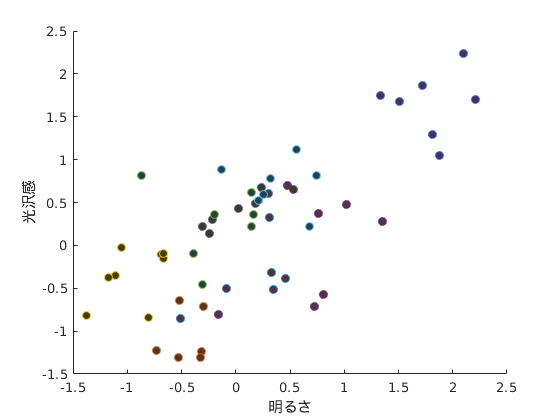
\includegraphics[width=11.0cm]{./img/ex3_DSD.png}
                \caption{Dragon形状のSD条件における明るさ感と光沢感の関係}
                \label{ex3_DSD}
            \end{figure}

            \begin{figure}[h]
                \centering
                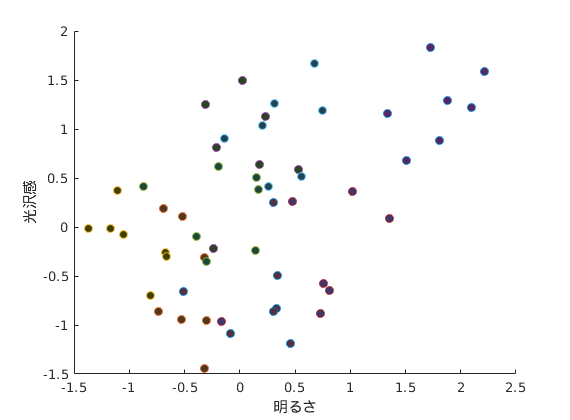
\includegraphics[width=11.0cm]{./img/ex3_BSD.png}
                \caption{Bunny形状のSD条件における明るさ感と光沢感の関係}
                \label{ex3_BSD}
            \end{figure}

            \newpage
            \begin{figure}[h]
                \centering
                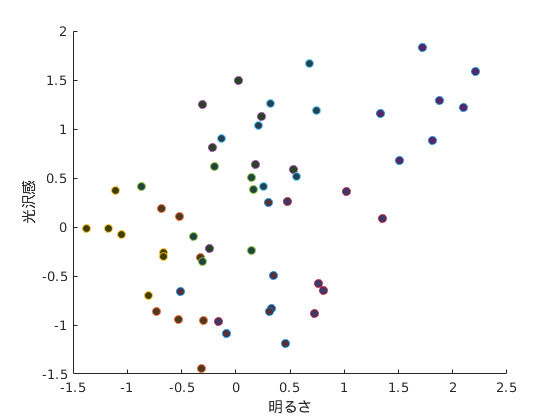
\includegraphics[width=11.0cm]{./img/ex3_DD.png}
                \caption{Dragon形状のD条件における明るさ感と光沢感の関係}
                \label{ex3_DD}
            \end{figure}

            \begin{figure}[h]
                \centering
                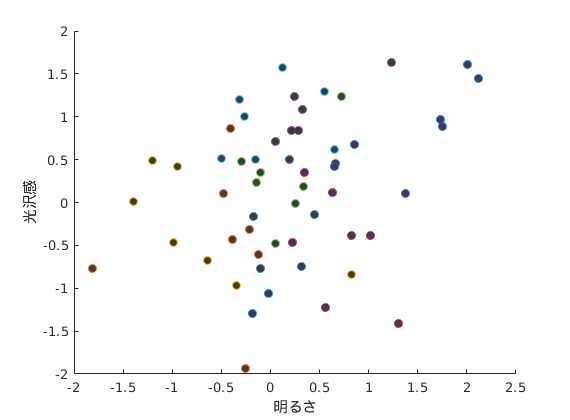
\includegraphics[width=11.0cm]{./img/ex3_BD.png}
                \caption{Bunny形状のD条件における明るさ感と光沢感の関係}
                \label{ex3_BD}
            \end{figure}

            \begin{table}[h]
                \centering
                \caption{各条件における光沢感と明るさ感の相関係数}
                \begin{tabular}{|l||c|c|} \hline
                                & SD       & D        \\ \hline \hline
                    Dragon      & 0.88   & 0.83   \\ \hline
                    Bunny       & 0.65   & 0.52   \\ \hline
                \end{tabular}
                \label{cc}
            \end{table}

            
            図\ref{ex3_DSD}から図\ref{ex3_BD}は,実験1と実験2の結果をそれぞれz-score化してから,それらの関係性を物体形状と条件ごとに散布図としてプロットしたものである.
            横軸は明るさを,縦軸は光沢感を表す.
            各点の色は実験で使われた9種類の色度を表している.
            また表\ref{cc}は各物体形状・着色条件における相関係数を表す.

            いずれの条件においても,明るさ感と光沢感の間には正の相関がみられた.
            ただし,相関の強さは条件によって異なっていた.
            具体的には,Dragon形状におけるSD条件,Dragon形状におけるD条件においては比較的強い正の相関が見られたが,これに比べてBunny形状におけるSD条件,Bunny形状におけるD条件の相関係数はやや小さい値となった.
            
            \newpage
            \begin{figure}[h]
                \centering
                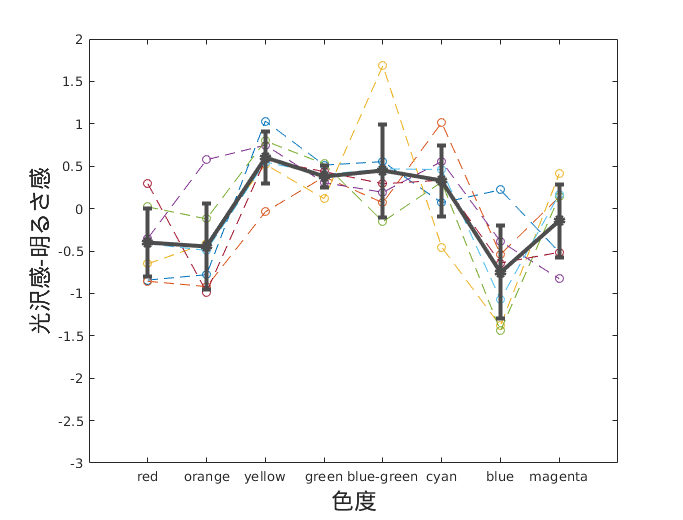
\includegraphics[width=11.0cm]{./img/ex4_DSD.png}
                \caption{Dragon形状のSD条件における明るさ感と光沢感の差分}
                \label{ex4_DSD}
            \end{figure}

            \begin{figure}[h]
                \centering
                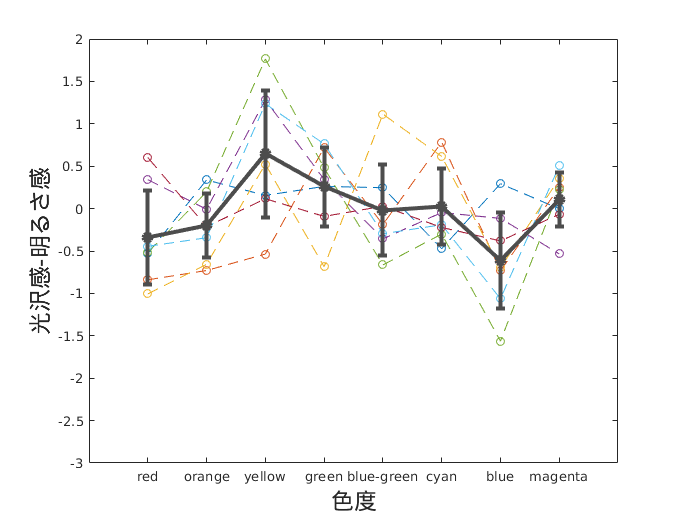
\includegraphics[width=11.0cm]{./img/ex4_BSD.png}
                \caption{Bunny形状のSD条件における明るさ感と光沢感の差分}
                \label{ex4_BSD}
            \end{figure}
            
            \newpage
            \begin{figure}[h]
                \centering
                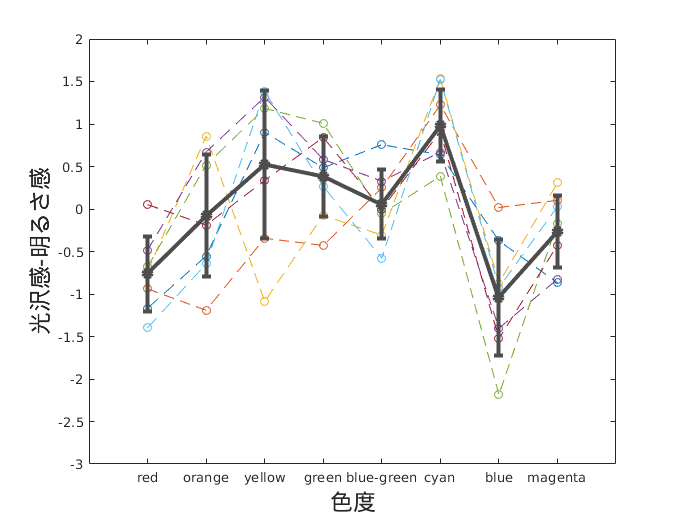
\includegraphics[width=11.0cm]{./img/ex4_DD.png}
                \caption{Dragon形状のD条件における明るさ感と光沢感の差分}
                \label{ex4_DD}
            \end{figure}

            \begin{figure}[h]
                \centering
                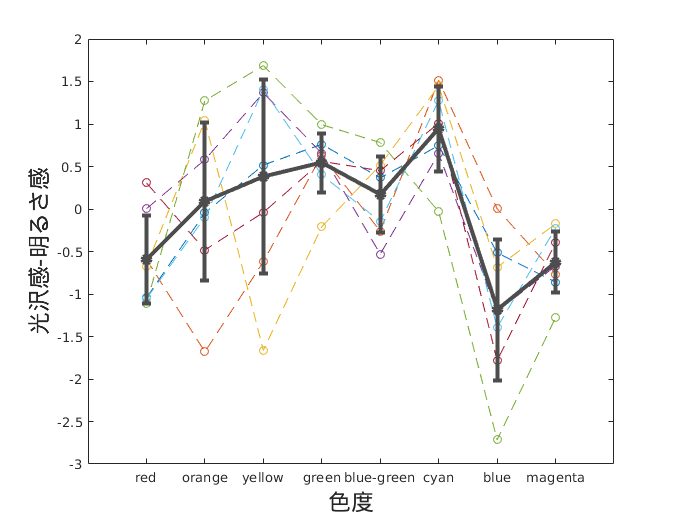
\includegraphics[width=11.0cm]{./img/ex4_BD.png}
                \caption{Bunny形状のD条件における明るさ感と光沢感の差分}
                \label{ex4_BD}
            \end{figure}

            明るさ感と光沢感の傾向の違いを詳細に検討する. 
            図\ref{ex4_DSD}から図\ref{ex4_BD}は,それぞれz-score化された光沢感(実験1の結果)から明るさ感(実験2の結果)を色度ごとに減算した結果を示す.
            各図は,物体形状とD/SD条件の組み合わせに対応する.
            いずれの図においても,横軸は色度,縦軸は明るさ感に対する光沢感を表す.
            破線グラフは各被験者の結果に対応し,色は被験者の違いを表す.
            また,黒実線のグラフは被験者平均のグラフを表し,誤差棒は95\%信頼区間を表す.
            この縦軸の値が正である場合は明るさ感に対し相対的に光沢感が高く,負である場合は明るさ感に対し相対的に光沢感が低いことになる.
            本論文では,便宜上この縦軸の値を「相対光沢感」と呼ぶことにする.
            
            全被験者間平均の結果に着目すると,物体形状とSD/D条件に関わらず,blueの相対光沢感は全色相で最小値となり,かつ有意に負の値となった.
            一方で,yellowとcyanでは,相対光沢感は正の値となり,特にD条件のcyanは有意に正の値となった.
            この結果は,特にblueやyellow,cyanの色度においては,色度付与による光沢感変化を明るさ感のみからでは予測できないことを示している.


        \section{考察}
        
            本実験の目的は,刺激全体の明るさ感が色度による光沢感増強効果を決定している可能性を検証することであった.
            実験結果では,物体形状やSD/D彩色条件に関わらず,光沢感と明るさの間に正の相関が得られた.
            この結果は,刺激全体から知覚される明るさ感が光沢感知覚に寄与していることを示唆している.

            しかしながら,明るさ感と光沢感の関係性が崩れる色相が存在した.
            例えば,yellowやcyanでは,H-K効果による明るさ感増強効果は弱いにも関わらず,光沢感は強く知覚された.
            反対に,blueでは,H-K効果による明るさ感増強効果が強いのに,光沢感はさほど高くなかった.
            この結果は,一部の色相においては色度付与による光沢感変化はその明るさ感からは予測できないことを示しており,これらの色相では明るさ感以外の要因が光沢感を変調したと考えられる.
            その要因の候補として,色度そのものが直接的に光沢感を変調させた可能性が考えられる.
            特にcyanの特性においてSD/D条件間では異なる傾向が見られたことから,拡散反射成分と鏡面反射成分の間の色差も光沢感に関する情報を有している可能性がある.

    \newpage